\label{ap:mcnp_fixed}

The calculation workflow requires the MOAA UIF and the \textit{mcnp} directory containing the MCNP input files for the burnup calculation, as shown in Figure \ref{fig:tree2}.

% Directory tree
\begin{figure}[htbp!]
  \begin{center}
    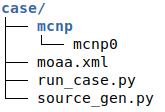
\includegraphics[width=0.23\linewidth]{figures/dh_case_directory}
  \end{center}
  \caption{Delayed heating case directory.}
  \label{fig:tree2}
\end{figure}

The delayed heating calculation requires two additional scripts: \texttt{run\_case.py} and \texttt{source\_gen.py}.
The user defines some of the calculation parameters in \texttt{run\_case.py}.
Some of these parameters include the name of the MOAA UIF, path to the MCNP neutron- and photon-transport input files, geometry cell numbers where to calculate the delayed heating, and photon-transport batch size - i.e., number of photon sources to be included in each photon-transport input file.
Section \ref{ap:batchsize} provides further details on the batch size.
If neutron and photon geometries are identical, the user must provide number of particles, and number of active and inactive cycles for the neutron-transport calculation.

% Execution
The execution of the workflow can be either interactive or batch mode from the command line by simply running \texttt{run\_case.py}.
An example of a submission script for execution on an \gls*{HPC} cluster can be found in Appendix \ref{ref:moaa-exec}, where instead of running MOAA, the user would run \texttt{run\_case.py}.
% Output
Upon successful execution, a \textit{.csv} is created summarizing the results.
The information is organized into rows and columns, where each row represents a decay step after shutdown, while each column contains the energy deposited by charged particles ($H_{ch}$), the energy deposited by photons ($H_{\gamma, Tr}$), and the total delayed heat ($H_T$), to mention a few.

% Description of the implementation
\section{Batch Size}
\label{ap:batchsize}

This work implements three different ways of calculating the delayed photon heating ($H_{\gamma, Tr}$):

\noindent
\textbf{First Method:} Runs one photon transport simulation for each cell contributing to the gamma heating.
For a system composed by $N$ cells, the method obtains the contribution of each cell independently ($^* \! F8_i$), and running $N$ simulations calculates the total gamma heating:
\begin{align}
H_{\gamma, Tr} [W] &= 1.6022 \times 10^{-13} \times \mathlarger{\sum}_{i \in N} \: ^* \! F8_i \times S_i
\end{align}

\noindent
\textbf{Second Method:} Obtains all contributions to the gamma heating of all cells simultaneously ($^* \! F8$), and then calculates the total gamma heating:
\begin{align}
H_{\gamma, Tr} [W] &= 1.6022 \times 10^{-13} \times \: ^* \! F8 \times \mathlarger{\sum}_{i \in N} S_i
\end{align}

\noindent
\textbf{Third Method:} Splits the calculation into $M$ simulations ($M < N$).
Each simulation includes $N_i$ cells ($N_i < N$).
The method calculates the contribution to the gamma heating of $N_i$ cells simultaneously ($^* \! F8_i$), and then calculates the total gamma heating:
\begin{align}
H_{\gamma, Tr} [W] &= 1.6022 \times 10^{-13} \times \mathlarger{\sum}_{i \in M} \left[ \: ^* \! F8_i \times \mathlarger{\sum}_{j \in N_i} S_j \right]
\end{align}


The first method runs $N$ photon-transport simulations, and in terms of computational expense, it is the most expensive.
However, this method allows to compare the magnitude of the different gamma heating contributors.
Additionally, each individual fixed-source simulation is completed in a matter of seconds.
Only when a system comprises a large number of cells, then, the computational expense becomes restrictive.

The second method runs only one photon-transport simulation, making it the least computationally intensive.
However, this method is only applicable for systems with a small number of cells due to MCNP limitations.
% To sample the position of the particles in a cell, MCNP uses the enclosing volume rejection method \cite{mcnp_primer_2011}.
To sample the position of the particles in a cell, MCNP uses the enclosing volume rejection method.
MCNP randomly samples the position within the enclosing volume, if the points fall within the cell, they are accepted.

To define the enclosing volume, MCNP uses the SI$_i$ card, for which $i$ is restricted to values between 1 and 999.
Our method defines additional SI cards to sample the cell where the particle is born and the energy of the particle for each cell.
If the enclosing volume is a box, it requires three additional SI cards for the position and one for the energy for each cell.
Overall, MCNP can sample the photon particles in only 248 cells within one input file, if the enclosing volumes are boxes or cylinders.
This reason motivated the development of the third method, which still allows to compute the total gamma heating with a considerably low computational expense.

Figure \ref{fig:atr-time2} displays the experiment heat production over time.
$H_{\gamma,Tr}$ was calculated for 761 and 4 independent photon-transport simulations.
Both results are identical within error bars.

% Describe the following figure
\begin{figure}[htbp!] %or H 
    \centering
    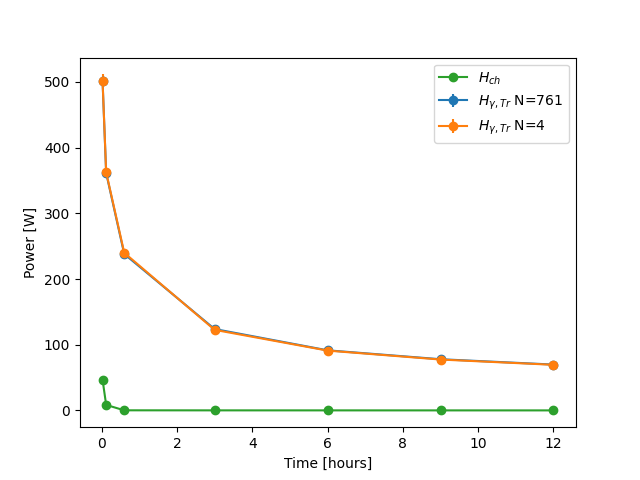
\includegraphics[width=0.55\linewidth]{figures/atr-decay-heat-time2}
    \hfill
    \caption{Heating rate over time in the ATR A1 experiment position for an aluminum sample.}
    \label{fig:atr-time2}
\end{figure}
